\begin{figure*}[hbt!]
\center
\begin{tabular}{@{}c@{}c@{}c@{}c@{}}
\hspace{-4.6cm}\panel{A} & \hspace{-5.2cm}\panel{B} & \hspace{-5.2cm}\panel{C} & \hspace{-2.3cm}\panel{D} 
\\[-0.6cm]
\raisebox{0.35cm}{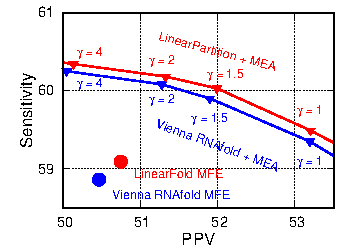
\includegraphics[scale=.8]{figs/LP_MEA_curves}} 
&
%\hspace{-0.5cm}
\hspace{-0.3cm}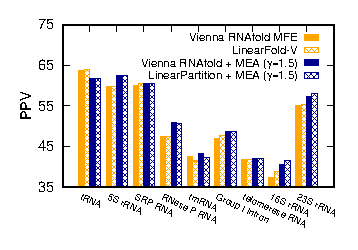
\includegraphics[scale=.93]{figs/MEA_vs_MFE_PPV} 
&
%\hspace{-0.5cm}
\hspace{-0.2cm}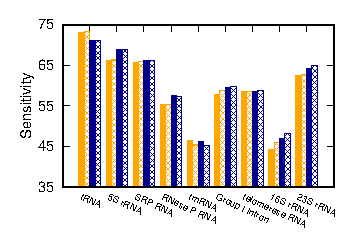
\includegraphics[scale=.93]{figs/MEA_vs_MFE_sens}  
&
\raisebox{.5cm}{\hspace{0.2cm}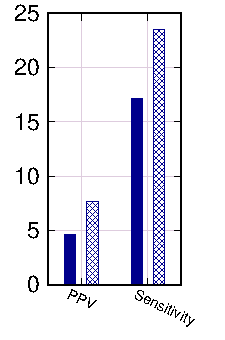
\includegraphics[scale=.56]{figs/bylen_500_mea}}
\\[-0.5cm]
\hspace{-4.6cm}\panel{E} & \hspace{-5.2cm}\panel{F} & \hspace{-5.2cm}\panel{G} & \hspace{-2.3cm}\panel{H} 
\\[-0.5cm]
\raisebox{0.35cm}{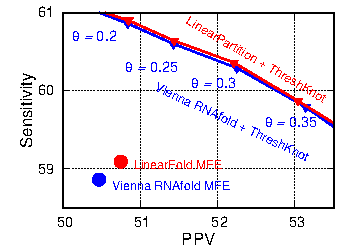
\includegraphics[scale=.8]{figs/LP_ThreshKnot_curves.pdf}}
&
%\hspace{-0.5cm}
       \hspace{-0.3cm}{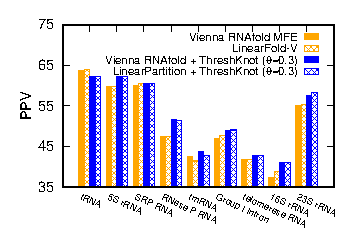
\includegraphics[scale=.93]{figs/new_ThreshKnot_vs_MFE_PPV}}
&
%       \hspace{-0.5cm}
      \hspace{-0.2cm}{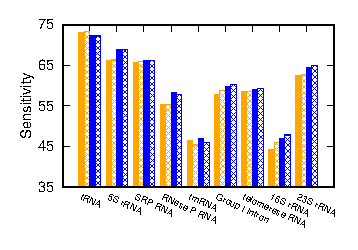
\includegraphics[scale=.93]{figs/new_ThreshKnot_vs_MFE_sens}}
              &
\raisebox{.5cm}{\hspace{0.3cm}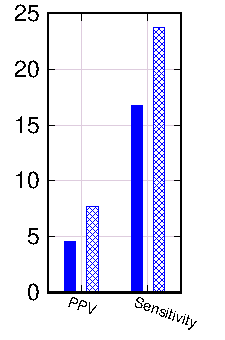
\includegraphics[scale=.56]{figs/bylen_500_threshknot} }
\vspace{-0.6cm}
\end{tabular} % A: specify MFE in label
\caption{Accuracy of downstream  predictions (MEA and \threshknot) using base pairing probabilities from \viennarnafold and \linearpartition
        on the ArchiveII dataset.
	{\bf A}: Overall PPV-Sensitivity tradeoff of MFE (single point) and MEA with varying $\gamma$
	%MFE is a single point, but
        (which can be tuned for higher sensitivity or PPV by adjusting $\gamma$).
	{\bf B} \& {\bf C}: PPV and Sensitivity comparisons of MEA structures for each family.
  {\bf D}: Accuracy comparison of long-distance base pairs (>500 \nts apart) in the MEA structures.
        {\bf E--H}: Same as {\bf A--D}, but using \threshknot predictions instead of MEA.
	%% {\bf D}: Overall PPV-Sensitivity tradeoff of \threshknot with varying threshold $\theta$.
	%% {\bf E} and {\bf F}: PPV and Sensitivity comparisons of ThreshKnot structures for each family.
        %	For easy comparison, {\bf A} and {\bf D} and also {\bf BCEF} are on the same scales.
        We conclude that MEA predictions based on \linearpartitionv are consistently better in both PPV and Sensitivity than
        those based on \viennarnafold for all $\gamma$'s,
        while \threshknot predictions based on those two are almost identical for all $\theta$'s.
        \linearpartitionv is  substantially better on long-distance base pairs in both MEA and \threshknot predictions.
	\label{mea}
        \vspace{-0.6cm}
}
\end{figure*}
